% \documentclass[12pt,a4paper]{article}
% \usepackage[top=3cm,bottom=2cm,left=3cm,right=2cm]{geometry}

\documentclass[
	% -- opções da classe memoir --
	article,			% indica que é um artigo acadêmico
	11pt,				% tamanho da fonte
	oneside,			% para impressão apenas no recto. Oposto a twoside
	a4paper,			% tamanho do papel. 
	% -- opções da classe abntex2 --
	%chapter=TITLE,		% títulos de capítulos convertidos em letras maiúsculas
	%section=TITLE,		% títulos de seções convertidos em letras maiúsculas
	%subsection=TITLE,	% títulos de subseções convertidos em letras maiúsculas
	%subsubsection=TITLE % títulos de subsubseções convertidos em letras maiúsculas
	% -- opções do pacote babel --
	english,			% idioma adicional para hifenização
	brazil,				% o último idioma é o principal do documento
	sumario=tradicional 
	]{abntex2}

\usepackage{lmodern}			  % Usa a fonte Latin Modern
\usepackage[T1]{fontenc}		% Selecao de codigos de fonte.
\usepackage[utf8]{inputenc} % Codificacao do documento (conversão automática dos acentos)
\usepackage{indentfirst}		% Indenta o primeiro parágrafo de cada seção.
\usepackage{nomencl}  			% Lista de simbolos
\usepackage{color}	  			% Controle das cores
\usepackage{graphicx}	  		% Inclusão de gráficos
\usepackage{microtype} 			% para melhorias de justificação

% \usepackage[brazil]{babel}
\usepackage{wrapfig}
\usepackage{hyperref}
\usepackage[alf]{abntex2cite}
\usepackage{xcolor}
\usepackage{array}
\usepackage{amsmath}
\usepackage{subcaption}
\usepackage{fancyhdr}

\usepackage[acronym,nolist,nonumberlist,nogroupskip,nonumbers]{glossaries}

% ----------- CONFIGURACOES E FORMATACAO ---------- %

\selectlanguage{brazil}
% \let\printacronyms\relax
% --- 
% Espaçamentos entre linhas e parágrafos 
% --- 
\setlrmarginsandblock{3cm}{3cm}{*}
\setulmarginsandblock{3cm}{3cm}{*}
\checkandfixthelayout


% O tamanho do parágrafo é dado por:
\setlength{\parindent}{1.3cm}

% Controle do espaçamento entre um parágrafo e outro:
\setlength{\parskip}{0.2cm}  % tente também \onelineskip

% Espaçamento simples
\SingleSpacing
% Retira espaço extra obsoleto entre as frases.
\frenchspacing 


\makeglossaries

% ----------- DEFINIÇÃO DAS SIGLAS COM GLOSSARIES ---------- %
% Defina suas siglas aqui, ANTES DE \begin{document}.
% O primeiro argumento é o rótulo (label), o segundo é a sigla curta, o terceiro é a descrição completa.
\newacronym{cad}{CAD}{Computer-Aided Diagnosis}
\newacronym{cnn}{CNN}{Convolutional Neural Network}
\newacronym{mlp}{MLP}{\textit{Multilayer Perceptron}}
\newacronym{ia}{IA}{Inteligência Artificial}
\newacronym{fmabc}{FMABC}{Faculdade de Medicina do ABC}
\newacronym{pasi}{PASI}{Psoriasis Area and Severity Index}
\newacronym{em}{EM}{espectro eletromagnético} 
\newacronym{etl}{ETL}{\textit{Extract Transform Load}}

% ---------- INICIO DO TEXTO --------------- %
\begin{document}


%titulo
% --- Informações de dados para CAPA e FOLHA DE ROSTO ---
\titulo{Detecção de psoríase vulgar em pacientes brasileiros por meio de um sistema computer-aided diagnosis baseado em visual transformers}
\def \theforeigntitle{}

\autor{Lucas Gargalhone Antunes Corrêa \textsuperscript{1} 
\and Gustavo Scalabrini Sampaio \textsuperscript{1}
\\ 
\textsuperscript{1}Faculdade de Computação e Informática (FCI) \\ Universidade Presbiteriana Mackenzie São Paulo, SP – Brasil \\ 
\\
\textsuperscript{2}Programa de graduação em Sistemas de Informação \\ Faculdade de Computação e Informática (FCI) \\ Universidade Presbiteriana Mackenzie São Paulo, SP – Brasil 
\\
\\
\url{lucasgargalhone@mackenzista.com.br}
\\
\url{gustavo.sampaio@mackenzie.br}}
\data{2025}
% ---

% ---
% Configurações de aparência do PDF final

% alterando o aspecto da cor azul
\definecolor{blue}{RGB}{41,5,195}

% informações do PDF
\makeatletter
\let\@fnsymbol\@arabic
\hypersetup{
     	%pagebackref=true,
		%pdftitle={\@title}, 
		%pdfauthor={\@author},
    	%pdfsubject={Modelo de artigo científico com abnTeX2},
	    %pdfcreator={LaTeX with abnTeX2},
		%pdfkeywords={abnt}{latex}{abntex}{abntex2}{atigo científico}, 
		colorlinks=true,       		% false: boxed links; true: colored links
    	linkcolor=blue,          	% color of internal links
    	citecolor=blue,        		% color of links to bibliography
    	%filecolor=magenta,         % color of file links
		urlcolor=blue,
		%bookmarksdepth=4
}
\makeatother

\maketitle


\thispagestyle{empty}

\vspace{1.0cm}
   
\renewcommand{\baselinestretch}{0.6666666}
{\bf Resumo.} Lorem ipsum dolor sit amet, consectetur adipiscing elit. Nam quis porttitor est. Nullam commodo tellus eros, nec feugiat erat venenatis at. In tristique elementum velit. Donec ac sem consectetur, eleifend leo id, tempor est. Cras in velit nec urna porttitor molestie sit amet et eros. Nulla volutpat, neque a consectetur consectetur, neque elit ultricies neque, eu bibendum sapien tellus a ante. Pellentesque nec auctor ante, eu iaculis enim. Donec blandit efficitur vulputate. Maecenas maximus nisi sit amet leo sollicitudin placerat. Morbi tristique, eros in semper pharetra, tellus nulla aliquet sapien, vitae hendrerit felis ipsum at felis. Quisque sed enim quis sem elementum lobortis vel id nisl.In cursus volutpat quam, et dictum nunc ultrices eu. Vivamus eget lobortis lacus, non viverra ligula. Morbi luctus massa eu venenatis bibendum. Morbi pharetra diam enim, ac bibendum nisi accumsan eu. Proin vitae malesuada velit. Duis in magna ac velit.
\begin{flushleft}
{\bf Palavras-chave:} {\it CAD, Neural Networks, CAD Microscopy, CNN, CAD intravital}
\\[2.5cm]
\end{flushleft}


{\bf Abstract.} Lorem ipsum dolor sit amet, consectetur adipiscing elit. Nam quis porttitor est. Nullam commodo tellus eros, nec feugiat erat venenatis at. In tristique elementum velit. Donec ac sem consectetur, eleifend leo id, tempor est. Cras in velit nec urna porttitor molestie sit amet et eros. Nulla volutpat, neque a consectetur consectetur, neque elit ultricies neque, eu bibendum sapien tellus a ante. Pellentesque nec auctor ante, eu iaculis enim. Donec blandit efficitur vulputate. Maecenas maximus nisi sit amet leo sollicitudin placerat. Morbi tristique, eros in semper pharetra, tellus nulla aliquet sapien, vitae hendrerit felis ipsum at felis. Quisque sed enim quis sem elementum lobortis vel id nisl.In cursus volutpat quam, et dictum nunc ultrices eu. Vivamus eget lobortis lacus, non viverra ligula. Morbi luctus massa eu venenatis bibendum. Morbi pharetra diam enim, ac bibendum nisi accumsan eu. Proin vitae malesuada velit. Duis in magna ac velit.\begin{flushleft}
{\bf Keywords:} {\it CAD, Neural Networks, CAD Microscopy, CNN, CAD intravital}
\end{flushleft}


\fancyheadoffset[L]{0pt} % Remove offset da esquerda
\fancyheadoffset[R]{0pt} % Remove offset da direita
\fancyfootoffset[L]{0pt}
\fancyfootoffset[R]{0pt}
\pagestyle{fancy}
\fancyhf{}
\fancyhead[LE,RO]{\small{\textit{XXI jornada de Iniciação Científica}}}
\fancyfoot[C]{\thepage}


%tese
% RESUMO
\thispagestyle{plain}

\vspace{1.0cm}
   
\renewcommand{\baselinestretch}{0.6666666}
{\bf Resumo.} Lorem ipsum dolor sit amet, consectetur adipiscing elit. Nam quis porttitor est. Nullam commodo tellus eros, nec feugiat erat venenatis at. In tristique elementum velit. Donec ac sem consectetur, eleifend leo id, tempor est. Cras in velit nec urna porttitor molestie sit amet et eros. Nulla volutpat, neque a consectetur consectetur, neque elit ultricies neque, eu bibendum sapien tellus a ante. Pellentesque nec auctor ante, eu iaculis enim. Donec blandit efficitur vulputate. Maecenas maximus nisi sit amet leo sollicitudin placerat. Morbi tristique, eros in semper pharetra, tellus nulla aliquet sapien, vitae hendrerit felis ipsum at felis. Quisque sed enim quis sem elementum lobortis vel id nisl.In cursus volutpat quam, et dictum nunc ultrices eu. Vivamus eget lobortis lacus, non viverra ligula. Morbi luctus massa eu venenatis bibendum. Morbi pharetra diam enim, ac bibendum nisi accumsan eu. Proin vitae malesuada velit. Duis in magna ac velit.
\begin{flushleft}
{\bf Palavras-chave:} {\it CAD, Neural Networks, CAD Microscopy, CNN, CAD intravital}
\\[2.5cm]
\end{flushleft}


{\bf Abstract.} Lorem ipsum dolor sit amet, consectetur adipiscing elit. Nam quis porttitor est. Nullam commodo tellus eros, nec feugiat erat venenatis at. In tristique elementum velit. Donec ac sem consectetur, eleifend leo id, tempor est. Cras in velit nec urna porttitor molestie sit amet et eros. Nulla volutpat, neque a consectetur consectetur, neque elit ultricies neque, eu bibendum sapien tellus a ante. Pellentesque nec auctor ante, eu iaculis enim. Donec blandit efficitur vulputate. Maecenas maximus nisi sit amet leo sollicitudin placerat. Morbi tristique, eros in semper pharetra, tellus nulla aliquet sapien, vitae hendrerit felis ipsum at felis. Quisque sed enim quis sem elementum lobortis vel id nisl.In cursus volutpat quam, et dictum nunc ultrices eu. Vivamus eget lobortis lacus, non viverra ligula. Morbi luctus massa eu venenatis bibendum. Morbi pharetra diam enim, ac bibendum nisi accumsan eu. Proin vitae malesuada velit. Duis in magna ac velit.\begin{flushleft}
{\bf Keywords:} {\it CAD, Neural Networks, CAD Microscopy, CNN, CAD intravital}
\end{flushleft}

% \newpage

% computa o indice
\makeindex

% SUMÁRIO
% \pdfbookmark[0]{\contentsname}{toc}
%   \tableofcontents*
% \cleardoublepage

% Lista de figuras
% \thispagestyle{empty}
%   \listoffigures
% \newpage

\pagenumbering{arabic}
  \section{Introdução}
A relação entre a computação e área da saúde está cada vez mais próxima, prova disso são as diversas aplicações da computação na medicina, desde plataformas de atendimento remoto (telemedicina) até sistemas de diagnóstico guiado por computador (\ac{CAD}).
Os sistemas \acs{CAD} podem ser compostos de diferentes técnicas da computação. Em pesquisas recentes, esses sistemas têm sido beneficiados pelo uso da \ac{IA}, uma área da computação que tem a intenção de replicar a inteligência humana. Uma subárea da \acs{IA} importante para os sistemas \acs{CAD} é a Visão Computacional, cuja meta é utilizar computadores para emular a visão humana, incluindo o aprendizado e a capacidade de fazer inferências e agir com base em informações visuais. Uma área que age em conjunto com a Visão Computacional é o Processamento Digital de Imagens, que geralmente está atribuída no estudo e aplicação de técnicas de mais baixo nível, como o realce de contraste e aguçamento de imagens \cite{gonzalez2008digital}.
Na dermatologia, existe uma lacuna entre pacientes de doenças de pele e a expertise necessária para lidar com eles \cite{Hameed2019}. Pessoas que vivem nas áreas rurais são as que mais se prejudicam por conta da falta de recursos, aponta pesquisa da Organização Mundial de Saúde (2015). Os sistemas \acs{CAD} são muito vantajosos nesses cenários, oferecendo um pré-diagnóstico de diversas doenças. Além disso, esses sistemas buscam proporcionar ao processo para definição da doença maior precisão, garantindo o tratamento adequado ao paciente e diminuindo custos operacionais (\cite{Hameed2019}, \cite{DAS2020119556}, \cite{Arora2021}. Uma doença dermatológica que pode ser analisada e diagnosticada por sistemas \acs{CAD} é a psoríase, a psoríase é uma doença inflamatória, crônica e recorrente que, de acordo com a Sociedade Brasileira de Dermatologia (2021), afeta a pele e articulações de mais de 5 milhões de brasileiros. Existem vários fenótipos dessa doença, sendo a mais comum a psoríase vulgar, presente em cerca de 90\% dos casos \cite{Griffiths2007}. Essa doença não apresenta risco à vida diretamente, porém traz diversas outras implicações para o paciente, desde coceira até sangramento na região. Estudos epidemiológicos identificaram também uma alta prevalência de fatores de risco cardiovascular em pacientes psoriáticos, característica importante, já que as doenças cardiovasculares como a síndrome metabólica, obesidade, hipertensão, \textit{diabetes mellitus}, resistência à insulina e a dislipidemia \cite{Miller2013} são a principal causa de morte, hospitalizações e atendimentos ambulatoriais em todo o mundo, inclusive em países em desenvolvimento como o Brasil \cite{Barroso2021}. 
A psoríase tem seu diagnóstico realizado inicialmente através de uma análise visual, ou seja, pela aparência clínica e distribuição da lesão. Identificada, ela é classificada como leve, moderada ou grave, sendo essa classificação baseada principalmente na superfície corporal afetada e no efeito da lesão no paciente. Diante disso, uma medida para a classificação da doença é a \ac{PASI}, que é dividida em dois passos, o primeiro é o cálculo da Área de superfície corporal (BSA) afetada com as lesões e o segundo passo consiste em avaliar o eritema (vermelhidão na pele), o endurecimento (espessura) e a descamação das lesões, de acordo com a Sociedade Brasileira de Dermatologia (2018).

\subsection{Objetivos}
O presente projeto tem como objetivo conduzir um estudo motivado pelo alto número de pacientes afetados pela psoríase, e também oportunidades de utilização de dados de pacientes brasileiros, para desenvolver um sistema \acs{CAD} dermatológico, baseado em um modelo de \acs{IA} utilizando técnicas de visão computacional, processamento digital de imagens e dados clínicos para diagnóstico de psoríase vulgar. Este trabalho dará início ao desenvolvimento de um sistema \acs{CAD} próprio,  utilizando imagens e dados clínicos de pacientes brasileiros. Essa característica é um dos pontos chaves do estudo, já que devido a fatores como a região, clima e exposição solar, a amostragem local é muito diferente comparada a outros trabalhos já propostos. Além disso,  essa combinação de dados não está presente em pesquisas anteriores, almejando assim atingir resultados superiores e mais consistentes para esse público. Para atingir essa meta serão trabalhados os seguintes objetivos específicos:
\begin{itemize}
  \item Definir e coletar as bases para o treinamento do modelo;
  \item Definir a arquitetura e treinar um modelo de \acs{IA} para a classificação de psoríase vulgar; usando imagens dermatológicas;
  \item Validar os resultados de desempenho do modelo treinado;
  \item Definir a arquitetura e treinar um modelo de \acs{IA} para a classificação usando os dados clínicos, que também devem compor o resultado da classificação das imagens;

  \item Validar os resultados de desempenho do modelo de dados clínicos;
  \item Analisar o ganho de desempenho com a combinação de imagens e dados clínicos;
  \item Construir de uma pipeline integrando os dois modelos;
  \item Analisar a viabilidade técnica de aplicação do método proposto em um produto real.

\end{itemize}

  \section{Referencial teórico}

Esta seção explora os fundamentos que sustentam o desenvolvimento de um sistema médico distribuído de alta disponibilidade.
Para contextualizar a proposta, serão abordados conceitos fundamentais sobre imagens microscópicas, o papel das redes neurais convolucionais na análise visual, a técnica de segmentação de imagens e uma revisão de trabalhos relacionados na área de sistemas CAD para análise de imagens médicas.

O avanço na criação dos algoritmos usados nos sistemas CAD tem sido enriquecido por contribuições de múltiplos campos do conhecimento, incluindo a filosofia, matemática, economia, neurociência, psicologia, engenharia da computação, linguística, teoria do controle e cibernética, destacando o caráter interdisciplinar que caracteriza o campo da IA. Segundo \cite{10.5555/1671238}, a Inteligência Artificial  é um campo da computação que se dedica ao desenvolvimento de agentes inteligentes, máquinas com aparente capacidade de raciocínio semelhante ao humano. Logo, a inteligência artificial, também envolve o treinamento desses agentes inteligentes. A subárea da IA que é responsável por explorar os algoritmos para o desenvolvimento desses agentes se chama aprendizado de máquina. 

Nesse campo de estudo, existem três abordagens distintas de aprendizados, o aprendizado supervisionado, onde o agente reconhece padrões mesmo sem ter recebido valores de saída explícitos; aprendizado por reforço, no qual o sistema aprende a partir de diversos estímulos, que funcionam como sinais para as decisões do agente, sejam estes negativos em caso de uma predição incorreta, ou positivos no caso de uma boa decisão; e por último, o aprendizado supervisionado, esse tipo de aprendizado é muito popular no treinamento das redes neurais convolucionais; nessa técnica de aprendizado, o agente recebe os dados de entrada e saída, e ao decorrer das iterações a IA aprende a função que mapeia a entrada com a saída \cite{haykin2009neural}.

A aplicação de algoritmos de aprendizado de máquina terá um impacto significativo neste estudo, permitindo que a rede reconheça os padrões e segmente a região das células. Será enfatizado a aplicação de uma categoria específica de algoritmos denominado aprendizado profundo (Deep learning (DL)), esse campo de estudo compreende uma vasta família de técnicas de aprendizado de máquina, nas quais as hipóteses são representadas por circuitos algébricos de elevada complexidade, com parâmetros de conexão ajustáveis. O termo ‘profundo’ refere-se ao fato de que esses sistemas geralmente estão organizados em camadas \cite{10.5555/1671238}. Esses circuitos conectados são conhecidos como redes neurais artificiais e são compostos por interconexões de um modelo matemático chamado \textit{perceptron}, que por sua vez tem seu funcionamento inspirado pelo neurônio humano.

\begin{figure}[h]
\centering\includegraphics[scale=0.4]{images/Figura-1-neuronio-artificial.png}
\caption{Exemplo do modelo perceptron \cite{imagemperceptron}.}
\label{fig: perceptron}
\end{figure}


O perceptron, demonstrado na Figura \ref{fig: perceptron}, foi inicialmente proposto por Frank Rosenblatt em 1957 como um classificador linear inspirado em neurônios biológicos, é uma unidade de processamento que recebe entradas \(x\) ponderadas pelos pesos \(w\), essa operação inicial pode ser representada como

\begin{equation}
  \(z = \sum_{i=1}^{n} w_i x_i\) \;.
  \label{eq:percetron}
\end{equation}

Posteriormente, a rede processa essas entradas por meio de uma função de ativação, a função de ativação tem a responsabilidade de amplificar o aprendizado do sistema, visto que por meio dessa função o neurônio será ativado ou não. A função de ativação aplica uma transformação não linear a saída da primeira operação \(z\), que é representada no final por \(\sigma = f(z + b)\), sendo \(b\) um termo de viés. Durante o treinamento, o perceptron ajusta seus pesos \(w_i\) com base no erro entre a previsão e o valor esperado. A regra de aprendizado é dada pela fórmula

\begin{equation}
  w_i = w_i + \Delta w_i
  \label{eq:Referencial}
\end{equation}

\noindent em que \(\Delta w_i = \eta(y_{esperado} - y_{previsto})\), sendo \(\eta\) o valor da taxa de aprendizado, que controla a magnitude da atualização dos pesos. Esse ajuste permite que ao decorrer das iterações o perceptron modifique suas conexões para melhorar seu desempenho em tarefas de calssificação \cite{haykin2009neural}. De maneira isolada, o perceptron possui a limitação de resolver apenas problemas linearmente separáveis, já a combinação de múltiplos perceptrons em camadas, conhecida como \textit{Multi Layer Perceptron} (MLP),  permite que esse modelo aproxime funções não lineares complexas.

\begin{figure}[h]
\centering\includegraphics[scale=0.75]{images/mlp.jpg}
\caption{Exemplo do modelo \textit{multi layer perceptron} (DTREG, 2024).}
\label{fig: mlp}
\end{figure}


Para \citeonline{haykin2009neural}, o MLP é um modelo baseado em aprendizado supervisionado, onde o objetivo é minimizar o erro na camada de saída. O MLP representa uma extensão do perceptron, cada camada do MLP realiza uma transformação não linear dos dados, assim, permite a captura de interações complexas entre as camadas. Exemplificado na figura \ref{fig: mlp}, as redes MLP são divididas em três partes: A camada de entrada, que possui a responsabilidade de receber os dados iniciais; as camadas intermediárias ou camadas ocultas (\textit{hidden layers}), que processam essas informações; e a camada de saída, onde é gerado os valores de saída da rede. Para atingir o objetivo de minimizar o erro, o sistema utiliza um algoritmo de retropropagação (\textit{backpropagation}) que foi proposto por \citeonline{Rumelhart1986-zt}.Esse algoritmo tem por objetivo ajustar os pesos ao longo das camadas, propagando o erro da camada de saída até as camadas intermediárias. Esse algoritmo utiliza a regra da cadeia para calcular o gradiente do erro em relação a cada peso da rede, facilitando o ajuste dos pesos para minimizar o erro. Esse algoritmo tem sua operação é divida em duas fases: a passagem para frente (\textit{forward pass}) e a passagem para trás (\textit{backward pass}). Na etapa da passagem para frente, a rede recebe uma amostra de entrada e propaga os valores através das camadas para gerar uma predição, ao final da rede, uma saída é gerada e comparada ao valor esperado, gerando um erro que será minimizado na próxima etapa. 

Contudo, no contexto de análise de imagens, há uma arquitetura de redes neurais mais especializada para entradas de imagens, essa arquitetura é denominada de redes neurais convolucionais (\textit{Convolutional Neural Network} (CNN)). As redes convolucionais são uma classe especial de redes neurais, desenvolvidas especificamente para o processamento de dados estruturados em grades, como imagens. As CNN, inicialmente propostas por \citeonline{6795724}, por meio de uma pesquisa para o reconhecimento de dígitos manuscritos, se tornaram uma das principais abordagens em visão computacional. Essa arquitetura de sistema envolve a composição das redes MLP com técnicas de processamento digital de imagens, como a convolução. A convolução é um processo de filtragem espacial (plano que contém os pixels da imagem), que consiste em aplicar o somatório do produto entre duas funções, a imagem e uma máscara ao longo da região que estas se sobrepõem, sendo a imagem uma função bidimensional f(i,j), em que i e j são as coordenadas, e a amplitude de f em qualquer par de coordenadas se refere a intensidade de cor naquele ponto, já a máscara é uma matriz de tamanho variado \cite{gonzalez2008digital}. 

\begin{figure}[h]
    \centering
    \includegraphics[scale=0.4]{images/redeconv.png}
    \caption{Exemplo rede neural convolucional (CORRÊA, 2024).}
    \label{fig: cnn}
\end{figure}

A figura \ref{fig: cnn} representa uma arquitetura típica de uma CNN, geralmente compostas por camadas convolucionais, de Pooling, totalmente conectadas e uma camada de saída. Cada uma dessas camadas realiza uma tarefa diferente, sendo as camadas convolucionais responsáveis pela atividade de extração de características, como bordas e texturas; a camada de Pooling é utilizada para reduzir a dimensionalidade dos dados; e por último, as camadas totalmente conectadas ou redes MLP que tem o mesmo funcionamento conforme apresentado anteriormente. 

A partir desse tipo de algoritmo, é possível se estender a tarefas mais avançadas que vão além da classificação de imagens, como por exemplo a segmentação de imagens. A tarefa de segmentação subdivide uma imagem em regiões ou objetos que a compõem. O nível de detalhe em que a subdivisão é realizada depende do problema a ser resolvido. O processo de segmentação deve parar quando os objetos ou as regiões de interesse de uma aplicação forem detectados \cite{gonzalez2008digital}. \citeonline{gonzalez2008digital} apontam que a segmentação de imagens é uma das tarefas mais difíceis no processamento de imagens, já que a precisão da segmentação determina o sucesso ou fracasso final dos procedimentos de análise computadorizada.

No contexto clínico, a utilização de dados visuais é indispensável para o diagnóstico da doença. A utilização desses sistemas é fundamental, visto que, diferente dos seres humanos, que são limitados à banda visual do espectro eletromagnético(EM), os aparelhos de processamento de imagem cobrem quase todo o espectro EM, variando de ondas gama a ondas de rádio. Esses sistemas podem trabalhar com imagens geradas por fontes que os humanos não estão acostumados a associar, como microscopia eletrônica, ultrassom e imagens geradas por computador \cite{gonzalez2008digital}.

Para o sistema proposto, o foco recai sobre a análise de dados obtidos através da microscopia, uma técnica fundamental para a visualização e o estudo detalhado de estruturas biológicas em nível celular. Na microscopia moderna existem algumas técnicas já bem estabelecidas, como a microscopia de fluorescência, em que é utilizada a luz ultravioleta para a geração dessas imagens - a tarefa básica do microscópio de fluorescência é utilizar uma luz de excitação para irradiar um espécime preparado e depois separar a luz fluorescente irradiante, muito mais fraca, da luz de excitação, mais intensa. A figura \ref{fig: fluomicro} apresenta um exemplo de microscopia de fluorescência. 

\begin{figure}[h]
  \centering\includegraphics[scale=0.18]{images/fluo-micro.png} 
  \caption{Imagem de microscopia fluorescente \cite{fluo-micro}.}
\label{fig: fluomicro}
\end{figure}

Dessa forma, só a luz de emissão atinge o olho ou outro detector. As áreas fluorescentes resultantes brilham contra um fundo escuro com contraste suficiente para permitir a detecção. Quanto mais escuro for o fundo do material não fluorescente, mais eficiente é o instrumento \cite{gonzalez2008digital}.

Em contraste, a microscopia óptica, também definido por \citeonline{gonzalez2008digital}, utiliza a luz visível transmitida ou refletida através da amostra e um sistema de lentes para ampliar a imagem, sendo essencial para a análise morfológica de células sanguíneas e tecidos, demonstrado na figura \ref{fig: opticalmicro}.

% \begin{figure}[h]
%   \centering\includegraphics[scale=0.18]{images/lung06.png}
% \caption{Imagem de microscopia óptica \cite{Schaadt2020}.}
% \label{fig: opticalmicro}
% \end{figure}

\begin{figure}[h]
  \begin{subfigure}{0.5\textwidth}
    \includegraphics[scale=0.16]{images/electron_micro} 
    \caption{Imagem de microscopia eletronica \cite{eletron-micro}}
    \label{fig: electronmicro}
  \end{subfigure}
% \hfill
  \begin{subfigure}{0.5\textwidth}
    \includegraphics[scale=0.16]{images/lung06}
    \caption{ Imagem de microscopia óptica \cite{Schaadt2020}.}
    \label{fig: opticalmicro}
  \end{subfigure}
\caption{Exemplo de amostras de microscopia}
\label{fig: microimg}
\end{figure}


E por último os microscópios eletrônicos - figura \ref{fig: electronmicro} - que operam como seus correspondentes óticos, mas utilizam um feixe concentrado de elétrons em vez de luz para criar a imagem de uma amostra, permitindo resoluções muito maiores devido ao menor comprimento de onda dos elétrons. Essas imagens microscópicas são essenciais para diversas análises científicas e médicas, e é justamente a partir delas que sistemas avançados, como os sistemas de detecção auxiliada por computador, podem ser treinados para identificar padrões e auxiliar no diagnóstico médico.

% \begin{figure}[h]
%   \centering\includegraphics[scale=0.2]{images/electron_micro.png}
%
%   \centering\includegraphics[scale=0.18]{images/lung06.png}
% \caption{Imagem de microscopia eletronica \cite{eletron-micro}.}
% \label{fig: electronmicro}
% \end{figure}


% Imagens microscopicas podem ser geradas de diferentes maneiras, entretanto no geral elas são formadas a partir do apoio de um dispositivo microscopico, que emite feixes de luz sob a materia sendo analisada, e todo esse processo é capturado por lentes com uma alta capacidade 

Os primeiros estudos sobre sistemas de detecção auxiliada por computador (CAD) e técnicas de análise quantitativa de imagens médicas por computador foram relatados na década de 1960. No entanto, foi na década de 80 que emergiu uma nova perspectiva, que assume que esses sistemas possam ser utilizados de maneira complementar aos profissionais da área da saúde e não para substituí-los. 

Portanto, o objetivo desses sistemas se torna ser uma segunda opnião para os médicos, para que estes façam a sua avaliação final. Alguns estudos ainda indicam que os sistemas CAD não devem necessáriamente apresentar uam precisão na classificação de doenças superior aos profissionais na área da saúde. No entanto, é fundamental observar que um maior desempenho desses sistemas resulta num valor final combinado mais otimizado, proporcionando maior eficiência entre a análise humana e computacional \cite{DOI2007198}. Atualmente, os sistemas CAD exploram diversas técnicas de inteligência artificial e visão computacional. Para auxiliar no desenvolvimento desta pesquisa, foram pesquisados artigos nas bases IEEE Explorer, Science Direct, Scopus, MDPI, utilizando as palavras chaves “CAD”, \textit{“Computer Aided System”}, \textit{“CAD convolution”}, \textit{“metastasis”}, “CAD cancer”, \textit{"microscopy"}, \textit{"metastasis"}, desses trabalhos se destacam os trabalhos de \citeonline{9152949}, \citeonline{BRINKER201911} e \citeonline{DASH2020106240}.

\citeonline{9152949}, apresenta uma abordagem do uso de aprendizado de máquina para o diagnóstico e estadiamento do cancêr pancreático (PC). O sistema foi desenvolvido utilizando uma técnica de \textit{ensemble learning}, que consiste em combinar o resultado de vários modelos para obter um valor final mais robusto. O \textit{ensemble} foi realizado envolvendo modelos do tipo \textit{support vector machine} (SVM). Nessa pesquisa, também foi abordado técnicas interessantes, como uma primeira etapa de segmentação e extração da região de interesse (ROI), outra atividade relevante foi a etapa de selação de características utilizando o algoritmo de seleção LASSO. O trabalho atingiu resultados relevantes, variando sua acurácia em torno de 75\% a 91.63\% em diferentes estágios da doença. Contudo, o trabalho ainda apresenta algumas limitações, como por exemplo os dados de treinamento, o qual é composto por apenas 54 pacientes, esse conjunto de dados pequenos é um dos fatores que dificulta a generalização do modelo, e também a distribuição desses dados, sendo que 39 pacientes desse conjunto possuem a doença e 15 são pacientes saúdaveis.

\citeonline{BRINKER201911} apresentou em sua pesquisa um sistema CAD especializado para dermatologia. Em seu trabalho, a classficação foi direcionada para o câncer melanoma, e obteve desempenho superior ao de dermatologistas na classificação das mesmas imagens. Para o desenvlvimento desse sistema, foi utilizado uma arquitetura de redes neurais convolucionais chamada de ResNet50, amplamente conhecida na literatura, porém com alguns ajustes como por exemplo, ao invés de utilizar a mesma taxa de aprendizagem para todas as camadas, o autor explorou diferentes taxas para diferentes camadas. Os dados utilizados para o treinamento e avaliação do modelo são de fontes de código aberto (\textit{open-source}) válidados por biópsia e foram avalidados por médicos profissionais, sendo selecionadas apenas as imagens entraram na categoria excelente, boa ou suficiente. Após o treinamento do modelo, os resultados obtidos evidenciaram sua eficácia. Com um intervalo de confiança (IC) de 95\%, o sistema alcançou uma sensibilidade de 82,3\% (IC 95\%: 78,3–85,7\%) e especificidade de 77,9\% (IC 95\%: 73,8–81,8\%). Em comparação, os dermatologistas apresentaram uma sensibilidade de 67,2\% (IC 95\%: 62,6–71,1\%) e especificidade de 62,2\% (IC 95\%: 57,6–66,9\%). Esses resultados reforçam o potencial dos sistemas CAD como ferramentas complementares no diagnóstico médico, especialmente em cenários de alta complexidade.

O trabalho de \citeonline{9097238} demonstra um novo esquema de sistema CAD para detecção de malária utilizando imagens microscópicas de uma fina camada de sangue. O seu sistema CAD parte do reforço de um modelo treinado composto por diversas camadas conectadas utilizado Functional Link Artificial Neural Network (FLANN) e Stacked Sparse Autoencoder (SSAE). O algoritmo FLANN é responsável por lidar com a redução de dimensionalidade dos dados, e a arquitetura SSAE é a caracteristica que possibilita o treinamento não supervisionado desse sistema, já que esse tipo de algoritmo se estende do tradicional modelo encoder-decoder, ele transforma e reconstroi a entrada. Com essa composição de diferentes técnicas, o autor atingiu resultados relevantes na detecção da doença, sendo 89.10\% de acurácia, 93.90\% de sensibilidade e 83.10\% de especificidade, além de atingir um tempo de detecção muito menor a que outros algoritmos sendo comparados na pesquisa.  


\citeonline{DASH2020106240} propôs uma abordagem utilizando redes neurais convolucionais organizadas de forma cascata. Nesse abordagem, foram concebidos dois desafios principais: a segmentação da lesão de psoríase e a avaliação objetiva de sua gravidade. O autor utiliza metodologias específicas para cada um dos desafios. Na etapa de segmentação da lesão, foi utilizado uma CNN do tipo U-Net modificada e para a tarefa de classificação foi utiliazada uma CNN do tipo VGG-16. Para o treinamento e avaliação do modelo, foram utilizados dados de fontes confiáveis validados por profissionais da área da saúde, além de métodos de validação cruzada como o k-pastas.


  \section{Metodologia}

O presente projeto apresenta o desenvolvimento de um sistema \gls{cad}, a partir de uma arquitetura de \textit{visual transformers}. Esse modelo terá a tarefa de lidar com a base de dados de imagens que foi fornecida pela \gls{fmabc}, composta de imagens de pacientes brasileiros afetados pela psoríase e pacientes com dermatite. A intenção dessa proposta é que a combinação de diferentes análises e informações traga um aumento na precisão desse tipo de sistema, fornecendo um suporte à tomada de decisão. Efetivamente, será implementada uma solução de ponta a ponta, que exigirá desde técnicas para o tratamento e preparo dos dados, até soluções para o refinamento do modelo de \gls{ia}.

A partir dos conceitos de redes neurais artificiais e \textit{transformers}, fica mais claro entender a construção dos modelos de \gls{ia}, que seguem um certo fluxo padrão, esse fluxo é conhecido como \textit{pipeline}. Os \textit{pipelines} de \gls{ia} envolvem todo o fluxo de atividades necessárias para o funcionamento apropriado do modelo. De modo genérico, este fluxo geralmente começa com atividades relacionadas à extração, transformação e carregamento dos dados, processo conhecido como \gls{etl}; no caso de modelos de \gls{ia} voltados a visão computacional, essa fase utiliza técnicas para preparar essas imagens a um modelo de \gls{ia}, geralmente envolvendo atividades relacionadas ao processamento digital de imagens. Além das transformações nas imagens é necessário realizar uma estratificação dos dados, uma parte deve ser separada para o treinamento da rede, enquanto a outra deve ser exclusivamente voltada para o teste da rede. A etapa seguinte envolve o treinamento da rede, essa etapa exige diferentes técnicas para o sucesso do modelo, entre essas técnicas estão a escolha de um algoritmo de otimização adequado ao problema, o uso de uma função de perda apropriada, ajuste correto dos hiperparâmetros da rede no treinamento. As subseções a seguir destacam cada uma das fases do \textit{pipeline} aplicado para o desenvolvimento do modelo.

\subsection{Coleta de dados}

A etapa de coleta de dados configura-se da responsabilidade de estabelecer formas consistentes de acesso aos dados fornecidos pela \gls{fmabc}, também deve garantir segurança e a integridade dessas informações. Para a realização da coleta de dados, foram desenvolvidos \textit{scripts} utilizando a linguagem de programação Go, uma ferramenta que ganhou muita popularidade devido ao seu desempenho. O desenvolvimento desses \textit{scripts} permitiram que todo o manuseio das informações fosse realizado de forma automatizada, além de coletar os dados, também envolvem tarefas como catalogação das informações.


\begin{figure}[h] % Ajuste largura
    \centering
    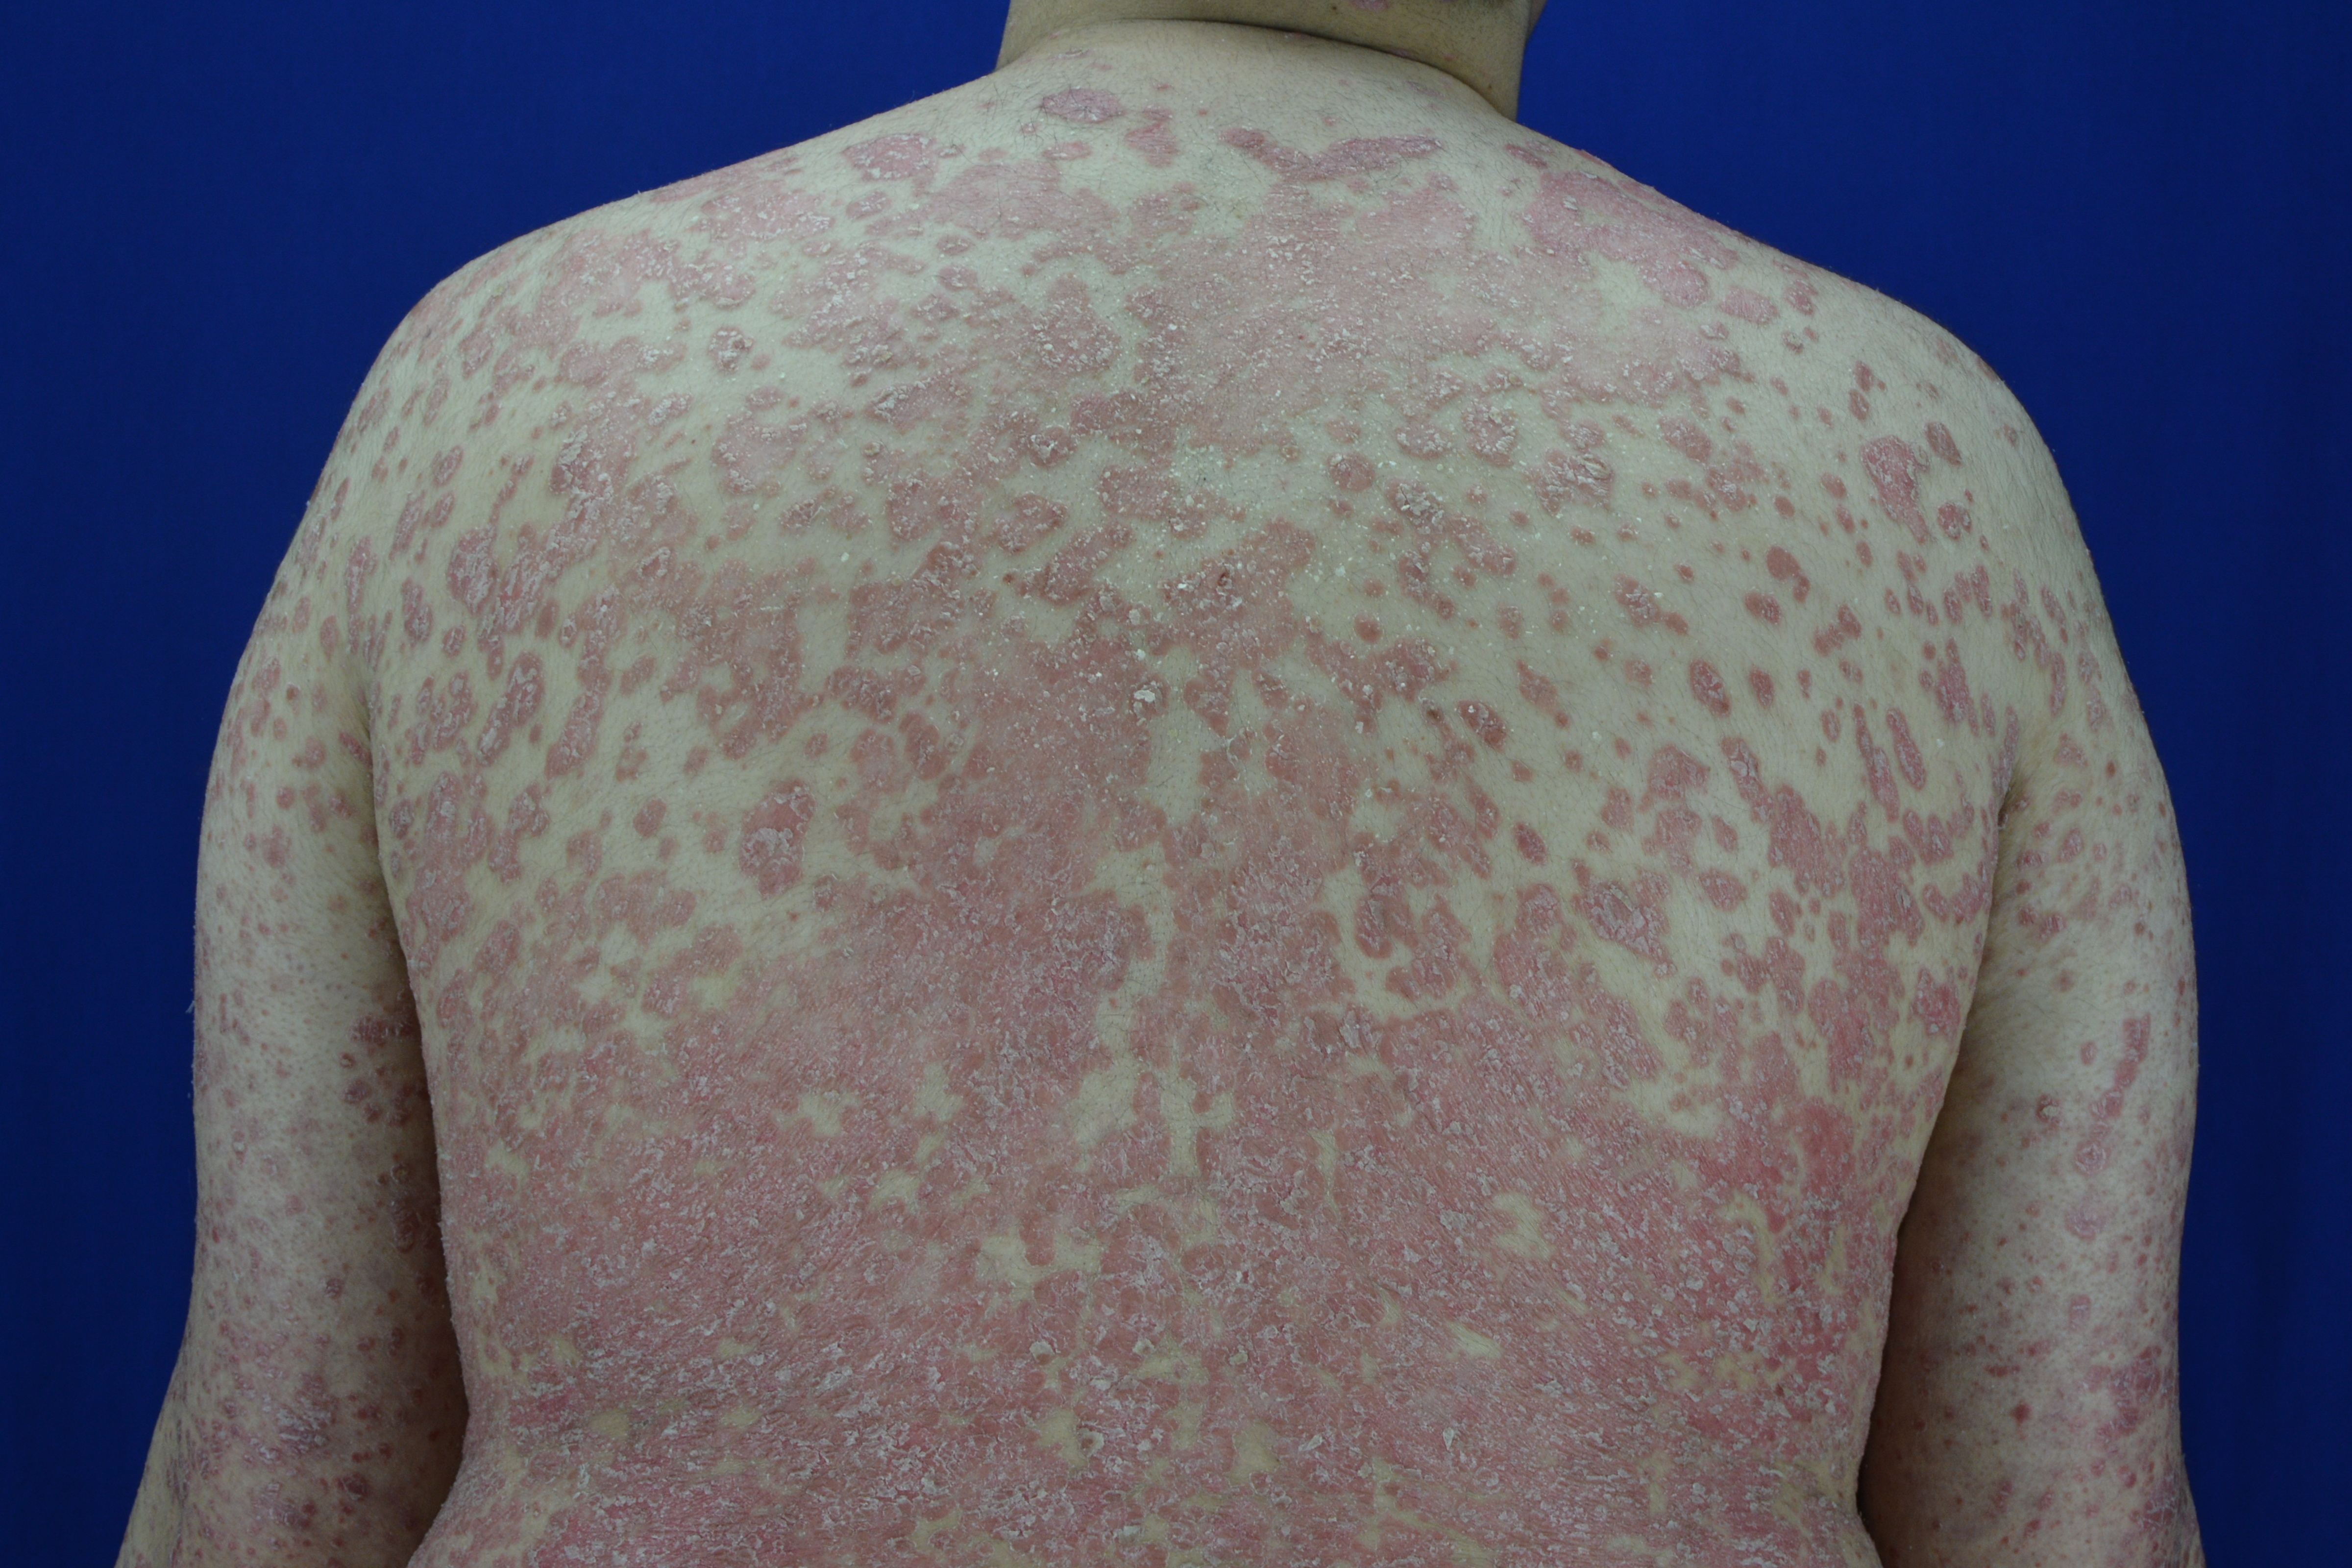
\includegraphics[width=0.6\textwidth]{images/dataset_example.jpg}
    \caption{Exemplo imagem de paciente com psoríase (FMABC, 2025)}
    \label{fig:ex-dataset}
\end{figure}

\subsubsection{Pré processamento}

Durante essa fase, foram estudadas quais seriam as técnicas aplicadas para preparar os dados coletados ao modelo, dados estes exemplificado na figura \ref{fig:ex-dataset}. Nessa fase foram encontrados alguns desafios, entre eles o primeiro é a limitação no número de amostragens recebidas pela instituição parceira e desbalanceamento entre as classes de dados, ou seja, na prática haviam trinta vezes mais imagens da categoria psoríase.

\begin{figure}[h] % Ajuste largura
    \centering
    \includegraphics[width=0.4\textwidth]{images/pre_processamento_psoriasis_jitter.png}
    \caption{Imagem de paciente com psoríase (FMABC, 2025)}
    \label{fig:ex-dataset}
\end{figure}

Antes do uso desses dados para o modelo, foi necessário uma inspeção manual sobre o dataset, que resultou na exclusão de 3000 imagens, devido a fatores como baixa qualidade, por exemplo imagens que estavam muito embaçadas ou com baixa resolução, e representação inadequada da classe, em que algumas fotografias que mostravam o corpo todo, e não a área lesionada. A utilização de tais imagens poderiam introduzir ruído e prejudicar a capacidade de generalização do modelos. 

Adicionalmente, para isolar a área de interesse, foi executado um pré-processamento específico para remover o fundo das imagens. Para este fim, foram desenvolvidos scripts customizados em \textit{Golang} que aplicavam duas estratégias de segmentação. A primeira estratégia visava remover o fundo azul predominante em muitas imagens do dataset. O script identificava os pixels dentro de um intervalo de cor azul pré-definido e os substituía por uma cor neutra. A segunda, mais refinada, utilizava um filtro baseado em intervalos de cor para isolar a área da pele e remover o restante da imagem.

Para lidar com as limitações mencionadas anteriormente, foram desenvolvidos e aplicados algoritmos de \textit{image augmentation}, esses algoritmos iteram sobre os dados fornecidos, e a partir destes, geram novos dados com filtros pré determinados. Neste trabalho, os filtros utilizados foram de \textit{random cropping}, que aplica um corte numa posição aleatória da imagem.

Outro desafio encontrado durante o pré processamento foram as dimensões das imagens, já que as imagens tinham dimensões por volta de 2400x3800 pixels, e esse tipo de arquitetura trabalha com entradas de 521x521 pixels, assim todas as tentativas de aplicar redimensionamento nas imagens não tiveram bons resultados, pois houve uma perda muito grande de qualidade dos dados, a alternativa encontrada para lidar com isso foi o uso já mencionado de \textit{random cropping}, pois o cropping descarta a necessidade de alterar os pixels da imagem, apenas usar um recorte de uma área aleatória.

No processo de \textit{data augmentation}, também foi aplicado a rotação de 50º graus nas imagens e \textit{flip} na horizontal e vertical, assim a mesma amostra porém em posição diferente poderia ser utilizada para treinamento da rede, o que enriqueceu o dataset e fortaleceu a capacidade de generalização do modelo. 
Além do aumento da base de dados, foram aplicadas transformações no domínio de cores das imagens. As imagens foram convertidas para o domínio de cor YCbCr, muitos \textit{softwares} de edição de imagens utilizam esse domínio para manipulação desses dados. A principal vantagem desse domínio é a separação da informação de luminância (canal Y) da informação de crominância (canais Cb e Cr)

Por fim, todas as imagens foram normalizadas, um passo importante para o treinamento de redes neurais. O procedimento de normalização consistiu em ajustar os valores dos pixels para o intervalo [0, 1], o que garante que a rede não seja afetada pela escala dos dados de entrada, promovendo uma convergência mais rápida e estável do modelo.

\subsection{Treinamento do modelo}

Para avaliar o desempenho do modelo de forma robusta e imparcial, foi utilizada a validação cruzada com \textit{k-folds} estratificada. O conjunto de dados foi dividido em \textit{folds}, garantindo que a proporção das classes fosse mantida em cada partição de treinamento e teste. Essa abordagem minimizou a dependência do modelo em relação a uma única divisão de dados.

A partir de um processo exploratório, em que foram aplicados diferentes testes com modelos de \gls{cnn} e \textit{Visual Transformers}, para identificar a configuração mais adequada para a tarefa de classificação binária de doenças de pele. As arquiteturas investigadas incluíram modelos de redes neurais convolucionais (\gls{cnn}), como VGG16 e ResNet152, e arquiteturas baseadas em transformadores, como Visual Transformers (\textit{ViT}) e Swin Transformers. Após uma análise comparativa, a arquitetura \textit{Swin Transformers} foi selecionada para o modelo final.

De modo a otimizar a busca por hiperparametros ideais para o objetivo proposto, foi utilizada uma técnica de \textit{Grid Search}, que consiste em testar e avaliar o desempenho de todas as combinações de parâmetros previamente fornecidos de forma automática. A Tabela \ref{tab: hiperparametros} apresenta os valores finais selecionados após a aplicação desta técnica.

A taxa de aprendizado foi explorada em um intervalo que incluiu valores como \texttt{[0.1, 0.01, 0.001]}, enquanto o decaimento de peso variou entre \texttt{[0.01, 0.001, 0.0001]}. O tamanho do lote também foi um parâmetro de otimização, testado com valores comuns na literatura como \texttt{[16, 32, 64]}. O valor final para o momento (\textit{momentum}) foi ajustado com base nos valores mais promissores, com o valor de \texttt{0.9} resultando no melhor desempenho. Após a avaliação exaustiva de todas as combinações, o conjunto de valores que obteve o melhor desempenho no conjunto de validação foi selecionado como a configuração final para o treinamento do modelo, conforme detalhado na Tabela \ref{tab: hiperparametros}.

\begin{table}[h]
    \centering
    \begin{tabular}{ll}
        \toprule
        \textbf{Hiperparâmetro} & \textbf{Valor} \\
        \midrule
        Otimizador              & SGD (\textit{Stochastic Gradient Descent}) \\
        Taxa de aprendizado     & 0.01 \\
        Momento (\textit{Momentum})     & 0.9 \\
        Decaimento de peso      & 0.001 \\
        Função de perda         & Entropia Cruzada Binária (\texttt{BCELoss}) \\
        Tamanho do lote         & 32 \\
        Número de épocas        & 40 \\
        Scheduler               & \texttt{ReduceLROnPlateau} \\
        \bottomrule
    \end{tabular}
    \caption{Hiperparâmetros finais utilizados no treinamento do modelo.}
    \label{tab: hiperparametros}
\end{table}


\subsection{Processo de análise dos resultados}

A avaliação do modelo incluiu análise quantitativa e qualitativa para compreender sua capacidade de tomada de decisão. Para tal, foram empregadas duas abordagens complementares: a análise de métricas de desempenho estatísticas e a interpretação visual por meio de mapas de calor.

O desempenho do modelo foi mensurado utilizando métricas de classificação padrão para problemas binários. Conforme os resultados desses métodos, foi possível analisar se o desempenho do modelo está de acordo com o esperado. Dentre as técnicas mais comuns, foram utilizadas métricas como acurácia, definida pela fórmula 

\begin{equation}
  acurácia = \frac{VP +VN}{VP + FN + VN + FP} \; ,
    \label{eq: acuracia}
\end{equation}

\noindent em que \(VP\) é a quantidade de verdadeiros positivos; \(VN\) é a quantidade de verdadeiros negativos; \(FN\) é a quantidade de falsos negativos e \(FP\) é a quantidade de falsos positivos. Em seguida, a métrica de precisão foi utilizada, determinada pela fórmula:

\begin{equation} 
  precisão = \frac{VP}{VP + VN} \; ,
  \label{eq: precisao}
\end{equation}

\noindent também, uma métrica de avaliação chamada sensibilidade, estabelecida pela fórmula:

\begin{equation}
sensibilidade = \frac{VP}{VP + FN} \; .
  \label{eq: sensibilidade}
\end{equation}

\noindent foi empregada a revocação (\textit{recall}), uma métrica que mede a capacidade do modelo de encontrar todas as amostras positivas, estabelecida pela fórmula:

\begin{equation}
revocação = \frac{VP}{VP + FN}
  \label{eq:revocacao}
\end{equation}

Por fim, o \textit{F1-Score}, que representa a média harmônica entre precisão e revocação, foi utilizado como uma métrica de equilíbrio para avaliar o modelo em cenários com classes desbalanceadas.

\begin{equation}
  F1 = 2 \cdot \frac{Precisão \cdot Revocação}{Precisão + Revocação}
  \label{eq:f1_score}
\end{equation}

Para estabelecer os mapas de calor e promover uma compreensão visual dos resultados do modelo, a ferramenta utilizada para essa tarefa foi o \textit{GradCam}, uma ferramenta de interpretabilidade que gera mapas de calor para qualquer camada convolucional de uma rede neural. Esses mapas destacam as regiões da imagem de entrada que mais influenciaram a decisão do modelo para uma determinada classe.

Na Figura \ref{fig:gradcam}, é apresentado um exemplo de um mapa de calor gerado pelo Grad-CAM para a classe Psoríase. A análise da imagem demonstra que as regiões de maior ativação da rede (indicadas pelas cores quentes, como amarelo e vermelho) correspondem diretamente à área da lesão dermatológica. Essa observação valida o comportamento do modelo, confirmando que ele não se baseia em ruídos ou em informações de fundo, mas sim nas características morfológicas da lesão, que são clinicamente relevantes para o diagnóstico.

\begin{figure}[h]
  \centering
  \begin{subfigure}[b]{0.45\textwidth}
    \centering
    \resizebox{5cm}{5cm}{%
      \includegraphics{images/nogradcam.jpg}%
    }
    \caption{Imagem original - Psoríase}
    \label{fig:gradcam-original-psoriase}
  \end{subfigure}
  \hspace{0.1cm}
  \begin{subfigure}[b]{0.45\textwidth}
    \centering
    \resizebox{5cm}{5cm}{%
      \includegraphics{images/test1-compesos.png}%
    }
    \caption{GradCAM - Psoríase}
    \label{fig:gradcam-heatmap-psoriase}
  \end{subfigure}
  
  \vspace{0.5cm}
  
  \begin{subfigure}[b]{0.45\textwidth}
    \centering
    \resizebox{5cm}{5cm}{%
      \includegraphics{images/nogradcam-arms.jpg}%
    }
    \caption{Imagem original - Psoríase}
    \label{fig:gradcam-original-dermatite}
  \end{subfigure}
  \hspace{0.1cm}
  \begin{subfigure}[b]{0.45\textwidth}
    \centering
    \resizebox{5cm}{5cm}{%
      \includegraphics{images/gradcamtestarms.png}%
    }
    \caption{GradCAM - Psoríase}
    \label{fig:gradcam-heatmap-dermatite}
  \end{subfigure}
  
  \caption{Resultados da análise GradCAM para classificação de psoríase e dermatite.}
  \label{fig:gradcam}
\end{figure}

% % --- Poderia ficar nos objetivos? ---
% % Além do desenvolvimento de um modelo que seja capaz de segmentar imagens microscópicas de células com alta precisão, esse trabalho também propõe a aplicação desse modelo num sistema destinado a uso médico. 


  % \section{Cronograma}

Para alcançar o objetivo proposto neste projeto de pesquisa, os objetivos específicos traduzidos em tarefas de desenvolvimento serão desenvolvidos. O cronograma descrito na tabela \ref{cronograma} apresenta a distribuição dessas atividades no tempo.

\begin{table}[h!]
\centering
\setlength{\arrayrulewidth}{0.8pt}
\setlength{\tabcolsep}{5pt}
\renewcommand{\arraystretch}{1.2}


\small
\centering\begin{tabular}{|p{9cm}|*{11}{c|}}
\hline
\textbf{Atividades} & \multicolumn{11}{c|}{\textbf{Meses}} \\
\hline
  &
\textbf{1} & \textbf{2} & \textbf{3} & \textbf{4} & \textbf{5} & \textbf{6} & \textbf{7} & \textbf{8} & \textbf{9} & \textbf{10} & \textbf{11} \\ 
\hline
Criação de uma pipeline de dados para o armazenamento e tratamento dos dados & x & x &   &   &   &   &   &   &   &   &   \\ \hline
Análise detalhada das técnicas em sistemas CAD                              &   & x &   &   &   &   &   &   &   &   &   \\ \hline
Construção de uma prova de conceito do modelo de CNN para avaliar a viabilidade das técnicas escolhidas &   & x &   &   &   &   &   &   &   &   &   \\ \hline
Análise dos resultados da prova de conceito do modelo e definição das técnicas para a construção do modelo &   &   & x &   &   &   &   &   &   &   &   \\ \hline
Construção do modelo de CNN                                                &   &   &   & x & x &   &   &   &   &   &   \\ \hline
Avaliação do modelo de CNN e ajuste de hiperparâmetros                     &   &   &   &   & x & x &   &   &   &   &   \\ \hline
Construção da prova de conceito de um modelo de MLP                        &   &   &   &   &   & x &   &   &   &   &   \\ \hline
Análise de resultados da prova de conceito do modelo de MLP e definição das técnicas para o desenvolvimento do modelo de MLP &   &   &   &   &   &   & x &   &   &   &   \\ \hline
Construção do modelo MLP                                                   &   &   &   &   &   &   & x & x &   &   &   \\ \hline
Testes com o modelo e ajustes de hiperparâmetros                           &   &   &   &   &   &   &   & x & x &   &   \\ \hline
Análise de precisão do modelo em relação ao modelo de CNN                  &   &   &   &   &   &   &   &   & x & x &   \\ \hline
Análise de viabilidade do sistema                                          &   &   &   &   &   &   &   &   &   & x &   \\ \hline
Elaboração de artigo científico com apresentação dos resultados            &   &   &   &   &   &   &   &   &   & x & x \\ \hline
Processo de submissão do artigo científico para periódico                  &   &   &   &   &   &   &   &   &   &   & x \\ \hline
\end{tabular}
\caption{Cronograma de atividades do desenvolvimento do projeto.}
\label{cronograma}
\end{table}






% --- Imagem do cronograma

%\begin{figure}[h]
%    \centering
%    \includegraphics[scale=0.5]{images/Cronograma.png}
%    \caption{Tabela 1: Cronograma de atividades do desenvolvimento do projeto}
%    \label{fig:enter-label}
%\end{figure}



  \section{Resultados e Discussão}

A rede treinada apresentou resultados relevantes e muito promissores. Um dos principais desafios encontrado durante o processo de desenvolvimento foi a complexidade de trabalhar com o dataset, além do pré-processamento, també foi necessário a remoção de certas imagens que não estavam adequadas para o treinamento da rede, devido a diversos fatores externos, como por exemplo qualidade da foto. Mesmo em um ambiente controlado não havia um padrão da maneira como os dados eram gerados, portanto diversas imagens necessitavam de análise individual. A tabela \ref{tab:db-table} indica algumas informações sobre o dataset utilizado para o treinamento do modelo após o pré-processamento. 

Após todo o tratamento do dataset houve uma diminuição expressiva do volume da base de dados, um pouco mais de 50\% de redução, esse fator também gerou outros desafios durante a fase de treinamento, como a falta de elementos representativos. A imagem abaixo é um exemplo do resultado final sendo alimentado na rede.

\newline
\begin{table}[h]
  \centering
  \label{tab:db-table}
  \begin{tabular}{|l|l|l|}
  \hline
  \multicolumn{1}{|c|}{\textbf{Label}} & \multicolumn{1}{c|}{\textbf{Amostras}} & \multicolumn{1}{c|}{\textbf{Porcentagem}} \\ \hline
  Psoríase                             & 1019                                   & 45.1\%                                  \\ \hline
  Dermatite                            & 1239                                   & 54.9\%                                  \\ \hline
  \multicolumn{1}{|c|}{\textbf{Total}} & \multicolumn{1}{c|}{\textbf{2258}}     & \multicolumn{1}{c|}{\textbf{100\%}}     \\ \hline
  \end{tabular}
  \caption{Distribuição do dataset após o processo de curadoria.}
\end{table}

Apesar da redução do volume de dados, o modelo alcançou um desempenho satisfatório. A Tabela \ref{tab:resultados_metricas} resume as métricas de avaliação obtidas no conjunto de teste. Observa-se que a acurácia de 93,78\% e o F1-Score de 0.9176\% indicam uma performance equilibrada, com a rede demonstrando robustez na distinção entre as classes.

\begin{table}[h]
  \centering
  \label{tab:resultados_metricas}
  \begin{tabular}{|l|c|}
  \hline
  \multicolumn{1}{|c|}{\textbf{Métrica}} & \textbf{Valor} \\ \hline
  Acurácia                               & 93,78\%           \\ \hline
  Precisão                               & 0.9211\%           \\ \hline
  Revocação                              & 0.9142\%           \\ \hline
  F1-Score                               & 0.9176\%           \\ \hline
  \end{tabular}
  \caption{Resultados das métricas de avaliação do modelo no conjunto de teste.}
\end{table}

Além da avaliação quantitativa, a interpretabilidade do modelo foi investigada por meio da técnica de Grad-CAM. A Figura \ref{fig:gradcam} apresenta um mapa de calor que ilustra as regiões de uma imagem de psoríase nas quais o modelo concentrou sua atenção para realizar a classificação. A análise visual desta figura confirma que a rede não se baseia em ruídos ou artefatos da imagem, mas sim nas características morfológicas da área lesionada (destacada em vermelho), o que fortalece a confiança em seus resultados e valida sua aplicabilidade clínica como ferramenta de apoio ao diagnóstico.


Durante o treinamento e a avaliação foram utilizadas diferentes técnicas que possibilitassem a análise do desempenho do modelo, a figura demostra as áreas de interesse que o modelo analisou para a classificação da doença. A partir dessa figura, é possível compreender como o modelo foi capaz de relacionar o contexto da região vermelha (área lesionada) com a classificação da doença psoriase




  \section{Conclusão}

Este trabalho apresentou o desenvolvimento de um sistema \gls{cad} para diagnóstico de psoríase vulgar baseado em \textit{Visual Transformers}, utilizando dados de pacientes brasileiros fornecidos pela \gls{fmabc}. O objetivo principal foi criar uma ferramenta de apoio ao diagnóstico capaz de distinguir entre psoríase vulgar e dermatite por meio de técnicas de visão computacional e processamento digital de imagens. Para atingir essa meta, foi implementado um \textit{pipeline} completo que envolveu desde a coleta e curadoria dos dados até o treinamento e avaliação de um modelo baseado na arquitetura \textit{Swin Transformers}. O modelo desenvolvido alcançou resultados promissores, com acurácia de 93,78\%, precisão de 92,11\%, revocação de 91,42\% e F1-Score de 91,76\%, demonstrando sua capacidade de classificação binária entre as duas condições dermatológicas estudadas.

Apesar dos resultados quantitativos satisfatórios, é fundamental destacar as limitações inerentes ao modelo, em grande parte, devido às características do dataset utilizado. A redução de mais de 50\% da base de dados original, embora necessária para garantir a qualidade das amostras, resultou em um volume limitado de imagens para o treinamento. 

Adicionalmente, as imagens foram capturadas em um ambiente controlado de laboratório universitário, o que as torna menos representativas de cenários clínicos reais, onde a variação de iluminação, qualidade da câmera e angulação é muito maior. Consequentemente, o modelo pode ter sua capacidade de generalização comprometida ao ser aplicado a imagens com características diferentes daquelas do conjunto de dados curado, como em um cenário de triagem em consultórios médicos. Tais limitações reforçam a necessidade de futuras pesquisas que utilizem um conjunto de dados mais diversificado, de maior volume e que simulem as condições do mundo real, a fim de aprimorar a robustez e a aplicabilidade clínica do modelo.

Apesar das limitações inerentes ao conjunto de dados, os resultados obtidos nesta pesquisa demonstram o potencial significativo do desenvolvimento de um sistema \gls{cad}.
A utilização de dados de pacientes brasileiros confere um valor estratégico ao modelo para a aplicabilidade em cenários clínicos nacionais. Além disso, este estudo serve como um ponto de partida para trabalhos futuros promissores. A evolução para um sistema capaz de realizar a segmentação automática da lesão ou a classificação da severidade da doença são direções de pesquisa que poderiam ampliar a funcionalidade e o impacto clínico da ferramenta.


  \newpage
  \renewcommand{\refname}{5 Referências}
\bibliographystyle{abntex2-alf}
\bibliography{Library}

\end{document}
